\chapter{The Scenarios Manager}
\label{chap:scenarios-manager}

\section{Running a Simulation}
Once a project has been developed, including the data to be used in it, and the model system has been configured and the parameters for the models estimated, the next step is to create and run a scenario.  In the eugene\_gridcell project, a baseline scenario has already been created and is ready to run.  To run this scenario, in the Scenario Manager, right-click with the mouse on the Eugene-baseline entry and select \verb#Run this Scenario#.  At this point, a frame should appear in the right hand side of the Opus window, as shown in Figure \ref{fig:opus-start-run}.

\begin{figure}[htp]
\begin{center}
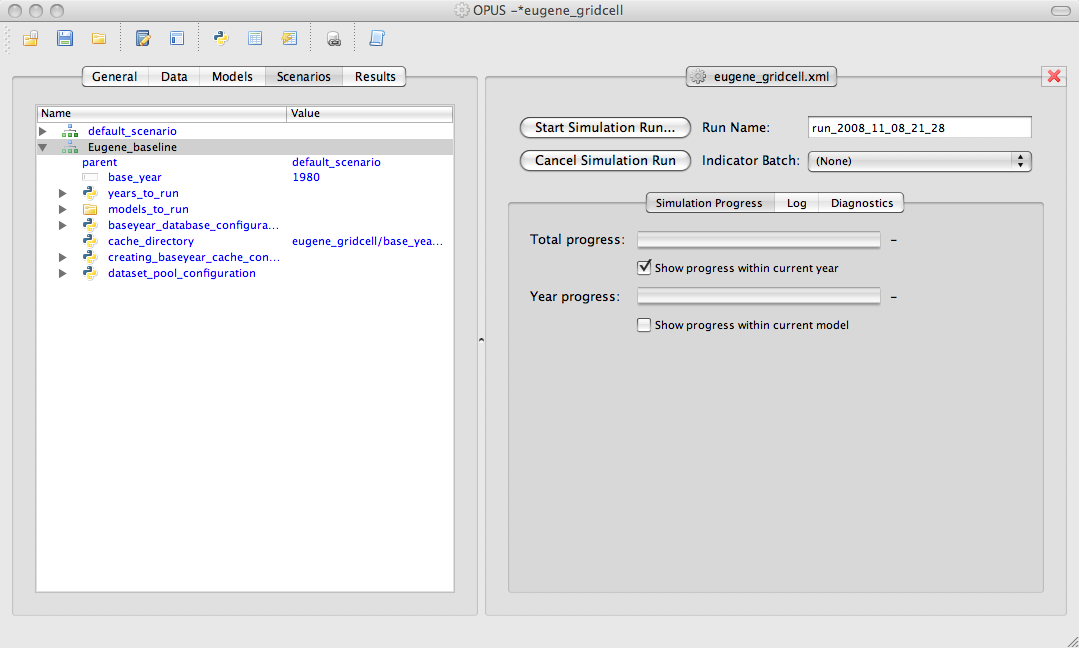
\includegraphics[scale=0.4]{part-gui/images/scenario-manager-start-run.png}
\end{center}
\caption{Starting a Simulation on a Scenario.xml}
\label{fig:opus-start-run}
\end{figure}

The frame on the right contains an option to start the run and an
option to remove the run from the queue.  The latter will remove this
new frame so that it is no longer available to run.  Start the run with
the first button option, labelled \verb#Start Model#.  The window will
now update as the simulation proceeds, with progress bars and labels
being updated to show the changing state of the system, such as what
year the model is simulating, what model is running, and even what part
of a model is running.  Figure \ref{fig:opus-running} shows the updated
window in this state.  Note that the \verb#Start Model#  button label
has now changed to \verb#Pause Model#.  If this is pressed while the
model system is running, a request to pause the model is triggered, and
once the current model in the model system is finished, the system
pauses until you take further action, like resume, or remove from
queue.

\begin{figure}[htp]
\begin{center}
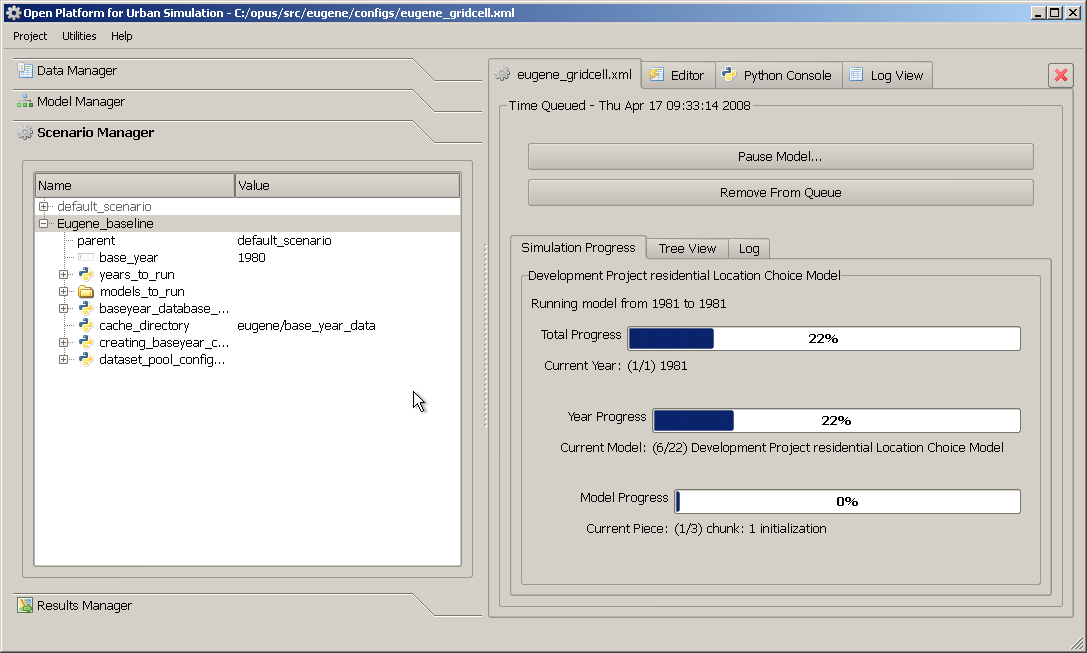
\includegraphics[scale=0.4]{graphics/opus-running.png}
\end{center}
\caption{Running a Simulation on a Scenario.xml}
\label{fig:opus-running}
\end{figure}

